% Chapter 3

\chapter{Literature Review} % Main chapter title

\label{review} % For referencing the chapter elsewhere, use \ref{Chapter1} 

\lhead{Chapter 3. \emph{Literature Review}} % This is for the header on each page - perhaps a shortened title

\section{Event Identification in News Text}
The event detection task \cite{allan2002topic} in the TDT program (Topic Detection and Tracking), led to significant advancements in the field of event-based organization of broadcast news. Some of the efforts in the TDT program focused on online event detection from continuous and real-time streams of textual news documents in newswires \cite{allan1998line,kumaran2004text}. While others explored the detection of past events from archived news documents \cite{yang1998study}. 

The textual content in news documents are different from the short informal text common in the realm of social media.  Most of these documents contain formal text with well-formed grammatical structures, enabling the researchers to rely on the state-of-the-art natural language processing techniques. Named entity extraction and Parts-of-Speech (POS) tagging are among the widely used techniques. Zhang et al. \cite{zhang2007new} extracted named entities and POS tags from textual news documents, and used them to reweigh tf-idf representations of these documents for the new event detection task. Filatova and Hatzivassiloglou \cite{hatzivassiloglou2003domain} identified named entities corresponding to participants, locations, and times in text documents, and then used the relationships between certain types of entity pairs to detect event content. Hatzivassiloglou et al. \cite{hatzivassiloglou2000investigation} used linguistic features (e.g., noun phrase heads, proper names) and learned a logistic regression model for combining these features into a single similarity value. Makkonen et al. \cite{makkonen2004simple} extracted meaningful semantic features such as names, time references, and locations, and learned a similarity function that combines these metrics into a single clustering solution. They concluded that augmenting documents with semantic terms did not improve performance, and reasoned that inadequate similarity functions were partially to blame. 

Extracting events from text has been the focus of numerous studies as part of the NIST initiative for Automatic Content Extraction (ACE) \cite{ahn2006stages,ji2008refining}. The ACE program defines event extraction as a supervised task, given a small set of predefined event categories and entities, with the goal of extracting a unified representation of the event from text
via attributes (e.g., type, subtype, modality, polarity) and event roles (e.g., person, place, buyer, seller). Ahn \cite{ahn2006stages} divided the event extraction task into different subtasks, including identification of event keyword triggers (see Chapter 2), and determination of event
coreference, and then used machine learning methods to optimize and evaluate the results of each subtask. Ji and Grishman \cite{ji2008refining} proposed techniques for extracting event content from multiple topically similar documents, instead of the traditional approach of extracting events from individual documents in isolation. In contrast with the predefined templates outlined by ACE, Filatova et al. \cite{filatova2006automatic} presented techniques to automatically create templates for event types, referred to as domains, given a set of domain instances (i.e., documents containing information related to events that belong to the domain). 

As already discussed, social media documents are extremely concise, noisy and lacks well-established grammatical structures. Therefore, the techniques used in these works are not suitable for identification of events from social media.  It has been shown that it is extremely challenging for the state-of-the art information extraction algorithms to perform efficiently and give accurate results for micro-blogs \cite{derczynski2013microblog}. For example, named entity recognition methods typically show 85-90\% accuracy on longer texts, but 30-50\% on tweets \cite{ritter2011named}. Therefore, new approaches had to be taken, leading to new techniques for detecting events in social media, which we discuss next.

%One of the goals of the EIIM framework presented in this thesis, is to identify and track event related content being generated in social media. However, the framework does not require detection of unknown events from real-time streams of social media messages. Instead it is provided with a predefined set of events along with predefined hashtags for the respective events, which are used for relevant data collection.

\section{Event Identification in Social Media}
While event detection in textual news documents has been studied in depth, the identification
of events in social media sites is still in its infancy. Several related papers explored the unknown event identification scenario in social media.
Weng and Lee \cite{weng2011event} proposed wavelet-based signal detection techniques for identifying
real-life events from Twitter. These techniques can detect significant bursts or trends
in a Twitter data stream. Sankaranarayanan et al. \cite{sankaranarayanan2009twitterstand}
identified late breaking news events on Twitter using clustering, along with a text-based
classifier and a set of handpicked news seeders. But they do not take into account the filtering of non-event content, which results in poor performance. Segregating the messages that have high likelihood of containing informative content from the ones with chances of having non-informative content are at the core of our work.  

% but, unlike our work in Chapter 4, they do not filter the vast
%amount of non-event content that exists on Twitter. This, unfortunately, results in poor
%performance, with very low precision scores compared with the precision achieved by our
%methods. Related to our work in Chapters 4 and 5, 



%As we discussed, such text-based and seeder-driven filtering of
%non-event data can be used to generate the event document stream we use in Chapter 5.

Petrovic et al. \cite{petrovic2010streaming} used locality-sensitive hashing to detect the first tweet associated with an event in a stream of Twitter messages. Rattenbury et al. \cite{rattenbury2007towards} analyzed the temporal usage distribution of tags to identify tags that correspond
to events. Chen and Roy \cite{chen2009event} used the time and location associated with Flickr image
tags to discover event-related tags with significant distribution patterns (e.g.bursts) in
both of these dimensions.
 
%
%%We use the general text-based classifier suggested in \cite{sankaranarayanan2009twitterstand} and a method for identifying top events suggested by Petrovic et
%%al. \cite{petrovic2010streaming} as baseline approaches in our evaluation of the unknown identification methods
%%of Chapter 4. While our work in the unknown event identification scenario focuses on timely, online, analysis, several efforts tried to address this task using retrospective analysis. 


Recent efforts proposed techniques for known identification of events in social media.
Many of these techniques rely on a set of manually selected terms to retrieve event-related
documents from a single social media site \cite{sakaki2010earthquake,yardi2010tweeting}. Our method of tracking an event is similar to this. We also use predefined hashtags to bootstrap the process of collecting data related to a known set of events. Sakaki et al. \cite{sakaki2010earthquake} developed
techniques for identifying earthquake events on Twitter by monitoring keyword triggers
(e.g., earthquake or shaking). In their setting, the type of event must be known a
priori, and should be easily represented using simple keyword queries. Benson et al. \cite{benson2011event} identified Twitter messages for concert events using statistical models to automatically tag artist and venue terms in Twitter messages.
Their approach is novel and fully automatic, but it limits the set of identified messages for
concert events to those with explicit artist and venue mentions. Importantly, both of these
approaches are tailored to one specific social media site. In contrast, we propose methods
for identifying social media documents across multiple sites with varying types of documents
(e.g., photos, videos, textual messages). Our goal is to automatically retrieve social media
documents for any planned event, without any assumption about the textual content of
the event or its associated documents. While not exclusively in the social media domain,
Tsagkias et al. \cite{tsagkias2011linking} extracted named entities and quotations from news articles, as
well as explicit links between news and social media documents, to identify social media
utterances related to individual news stories. In contrast with their well formed, lengthy
textual documents and explicitly linked content, content in our known event identification
setting (Chapter 6) is brief and often noisy, and generally does not contain explicit links to
social media documents.

\section{Information Quality in Social Media}

\section{Ranking and Summarization of Short Textual Social Media Posts}
There are many web hosted applications that supplements the default search provided by Twitter in order to effectively retrieve relevant and high quality tweets from different perspectives\footnote{\tiny http://mashable.com/2009/04/22/twitter-search-services}. On going through these services we found that the most commonly used criteria for ranking tweets are recency, popularity based on retweets and favorite counts, authority of the users posting the tweets and content relevance. Twitter itself uses the popularity of the tweets and features mined from the profile of the users in order to provide personalized search results ordered by recency\footnote{\tiny https://blog.twitter.com/2011/engineering-behind-twitter\%E2\%80\%99s-new-search-experience}. A study of different state-of-the-art features and approaches commonly used for ranking tweets has been documented by \cite{damak2013effectiveness, nagmoti2010ranking}. Seen\footnote{\tiny http://seen.co} is a new state-of-the-art platform that uses a proprietary algorithm named \textit{SeenRank} for ranking event related tweet content for presenting event highlights and summaries. In this work, we consider \textit{SeenRank} as one of our baselines. As the number of retweets of a tweet is widely used for ranking, we also use it as one of our baselines. In the context of our work we name the ranking scheme as \textit{RTRank}

Apart from the existing real-world search applications, several adaptations of \textit{PageRank} \cite{page1999pagerank} has been proposed by the scientific community for ranking tweets and users in Twitter \cite{weng2010twitterrank,tunkelang2009twitter, hallberg2012adaptation}. 
%TweetRank \cite{hallberg2012} is one such adaptation that ranks tweets by taking into account the direct relationships between tweets in the form of retweets and replies, as well as indirect follower-friend relationships, and usage of similar hashtags. 
Various learning to rank approaches have been used for ordering tweets retrieved for a given query in terms of their relevance and quality \cite{duan2010empirical,mccreadie2013relevance,vosecky2012searching}. None of these ranking techniques have been devised for event-specific content. An attempt to solve a similar problem presented in this paper was made by \cite{becker2011selecting}. They represented tweets of an event in a cluster and calculated the similarity of individual tweets with the centroid of the cluster. Then they ranked the tweets based on the decreasing value of their similarity. We use this approach as one of our baselines.

%Research on summarizing, discovering, or otherwise presenting social media content has
%gathered recent attention. The task of social media summarization is related to our content
%, but instead of selecting a set of potentially disconnected
%messages, it aims to construct a coherent summary representation. Several eorts [CP11;
%SHK10] considered ways to summarize a set of social media documents related to a specific
%topic. Sharifi et al. [SHK10] proposed approaches for summarizing a set of Twitter messages
%that were retrieved in response to a keyword query. They used graph-based phrase
%reinforcement and tf-idf techniques to produce very short summaries, which often consist
%of fewer than 10 words. Chakrabarti and Punera [CP11] proposed techniques for summarizing Twitter messages for events. They used Hidden Markov Models to segment the set
%of messages into sub-events, and then selected key messages from each interesting subevent,
%to include in the overall summary. This approach, as the authors note, is geared
%towards structured, long-running events and its effectiveness has not been determined for
%short events such as concerts or festivals.

\section{Entity Resolution}

Entity resolution has been known for more than five decades as the record linkage or the record matching problem in the statistics community \cite{fellegi1969theory,newcombe1959automatic,herzog2007data}. In the database community, the problem is defined as merge-purge \cite{hernandez1998real}, data de-duplication \cite{sarawagi2002interactive,ananthakrishna2002eliminating}, and instance identification \cite{wang1989inter}. In the Artificial intelligence community, this problem is described as database hardening \cite{cohen2000hardening}, and name matching \cite{bilenko2003adaptive}. The names co-reference resolution, identity uncertainty, and duplicate detection are also commonly used to refer to the same task \cite{elmagarmid2007duplicate}. The term Entity Resolution (ER) first appeared in publications by researchers at the Stanford InfoLab led by Hector Garcia-Molina and is defined as the process of identifying and merging records judged to represent the same real-world entity \cite{garcia2006pair}. In the context of the work presented in this thesis a pre-defined real-life event is considered as an entity. For detailed definition of an event please refer Chapter \ref{events}.

Despite the differences in nomenclature used by these authors, the ER process actually comprises five major sub-tasks or activities \cite{talburt2011entity} which are
\begin{enumerate} 
\item	\textit{Entity reference extraction} – locating entity references in unstructured textual information
\item	\textit{Entity reference preparation} – profiling, standardizing, cleaning, and enhancing reference information in preparation for resolution
\item	\textit{Entity reference resolution} – the process or algorithm for determining when references are equivalent, often through direct matching of attributes
\item	\textit{Entity identity management} - creating and maintaining persistent data structures that represent the identities of external entities, the focus of the proposed research
\item	\textit{Entity relationship analysis} – exploring relationships among distinct entities such as household relationships or shared communication
\end{enumerate}

The \textit{Event Identity Information Management} Life Cycle (Chapter \ref{eiim}) as proposed in this thesis reflects and implements all of the above activities. Historically the focus of ER research has been on Activity 3, the methods for carrying out the resolution process itself. The majority of published research literature falls into this area. The first formal model for resolution was the Fellegi-Sunter Model of Record Linkage \cite{fellegi1969theory}, which uses a decision-theoretic approach establishing the validity of principles first used in practice by Newcombe \cite{newcombe1959automatic}.  This was followed by the Stanford Entity Resolution Framework (SERF) developed at the Stanford InfoLab \cite{benjelloun2006generic}.  The SERF Model formalizes the generic ER problem as the interaction of two functions for comparing and merging records as black-boxes and defines the conditions required for these functions to give a unique ER result. It also formulates a family of so called ``Swoosh" algorithms (G-Swoosh, R-Swoosh, and F-Swoosh) for carrying out the ER process. With the rise of big data a distributed algorithm D-Swoosh \cite{benjelloun2007d}, was also proposed that can be implemented in a distributed environment. More recently the Talburt-Wang Algebraic Model of ER has been proposed \cite{talburt2007algebraic} that views ER as a problem of partitioning a given set of references. 
 
In addition to research on Activity 3, there has also been extensive research in the area of information extraction (IE) that is directly related to the ER Activity 1, reference extraction. The task of entity extraction is also more relevant to social media, due to the unstructured nature of the content. One of the main emphases in the realm of unstructured textual content for last two decades has been in the task of extracting named entities and categorizing them into types. Competitions like MUC (Message Understanding Conference), CoNLL (Conference on Computational Natural Language Learning) and ACE (Automatic Content Extraction) spearheaded the development of new techniques in this domain. This led to the development of sophisticated tools like Stanford NER \cite{finkel2007named}, OpenNLP \cite{baldridge2005opennlp}, GATE \cite{cunningham2002gate}, LingPipe \cite{baldwin2003lingpipe} and NLTK \cite{bird2006nltk}. Variety of techniques ranging from hand-coded rules, automatic rules, to statistical machine learning techniques like hidden Markov models, maximum entropy and conditional random fields have been proposed. A comprehensive survey of the techniques could be found in \cite{piskorski2013information,sarawagi2008information}. A study of various efforts in extracting information from micro-blogs could be found in \cite{hua2012information} and a survey of named entity recognition and classification could be found in \cite{nadeau2007survey}. Efforts have been made by the industry in building crowd sourced knowledge bases like freebase \cite{bollacker2008freebase} and dbpedia \cite{auer2007dbpedia} for the purpose of entity extraction. A recent effort from the industry for extracting entities from social media and building scalable knowledge bases for doing so has been documented in \cite{deshpande2013building,gattani2013entity}. The rise of online social networks, has also motivated new research into the ER Activity 5, entity relationship analysis \cite{bilgic2006d}. With the rise of big data, the modern trend is to perform entity resolution process in humongous volumes of data and scale it horizontally \cite{kolb2012dedoop}. In spite of the recent efforts in the field of entity extraction and resolution from unstructured text, there is no generic framework that solves the problem of persistently collecting and managing entity identity information from social media. The development of Event Identity Information Management from social media is a pioneering effort in the field of entity resolution and would create new avenues of research. As already discussed in the applications (Chapter \ref{applications}), it would open new doors in the field of social media data integration, cyber security, online payment and social media analytics.

Traditionally, identity resolution and management (Activity 4) has been a subject of system administration and management of user identities in large organizations. For the first time \cite{zhou2011entity}, showed the intersection of identity management, master data management and entity resolution could be used for managing identities of real-life entities in information systems, that could further play an important role in data integration and information quality. Entity identity management in social media mainly comprises of resolving and integrating profiles of the same person in social networking websites. The FOAF project has been playing an important role in all such efforts \cite{bouquet2010entity,bortoli2007foaf,raad2010user}. A very nice endeavor has been made by the OKKAM project for integrating and managing the multiple entity identifiers in various knowledge bases across the Internet \cite{bouquet2006okkam}. To our knowledge, we are the first to propose a framework for collecting and extracting identity information of events from social media and use the concepts of entity identity management and entity resolution for persistently managing their identities with respect to time.

%Because the focus of this research is on ER Activity 4, entity identity management, the detailed review of the literature around ER Activities 1, 2, 3, and 5 has been placed in Appendix A.
%In reviewing the literature of ER activity 4, most the references for identity management are related to cyber-security.  These publications generally fall into two main categories.  In the first category are papers that look at the problem of issuing information system users with credentials and unique identifiers during an initial registration phase.  In the second are those that focus on issues around authenticating users and controlling their access to services and resources based on their identifiers and credentials during the service operation phase (Josang & Pope, 2005). Some of the literature discusses “revocation” which is the process of rescinding and identity that has been granted as part of identity management (Slone, 2004). 
%The primary objective of the proposed research in entity identity management is to understand how identity is represented within an information system and how different representations can lead to different ER outcomes.  Currently there appears to be gap between the concepts of ER identity management and identity management in cyber-security.  A potentially important contribution of the proposed research is to help close that gap.  One of the reasons that this gap exists is that in both research and practice the focus is almost entirely on the algorithmic aspects of the resolution process such as matching, transitive closure, blocking, and indexing.  In most systems the identity information created during the resolution process is transient and discarded at the end of the process.  Therefore little attention has been paid to identity management as part of the ER process itself.
%Another potential contribution of the research is to help the designers and developers of ER systems understand how EIM structures and processes support the capture and storage of identity information and persistent entity identifiers, i.e. identifiers that do not change from process to process.  With the notable exception of Acxiom® AbiliTec®, almost no commercial ER systems provide EIM support or provide persistent entity identification.
%Those references related to identity and that are not directly related to cyber-security generally fall into the areas of philosophy, logic, and mathematics.  Identity is defined as (Merriam-Webster): 1. sameness of essential or generic character in different instances; 2. the distinguishing character or personality of an individual; 3. the condition of being the same with something described or asserted.  In ER and identity management, an identity is a representation of an entity in a specific application domain (Josang & Pope, 2005), which is also called surrogate identity in this research. If the entity is person, an identity could be a certain body of information about that particular person which serves as a representation of the real person in certain systems. Much of the literature related to the definition and understanding of identity comes from the areas of philosophy, logic, and mathematics.  
%Identity is not an object, but a binary relation of a special sort that logicians call an equivalence relation, which means that it has three features (Castellani, 2003):
%•	Reflexivity: For all x, x=x
%•	Symmetry: For all x and y, if x=y then y=x
%•	Transitivity: For all x, y, and z, if x=y and y=z then x=z
%In the above, the symbol “=” means is identical to, and the variables ‘x’, ‘y’, and ‘z’ are intended to range over any members (if in a set) whatsoever.  The same conditions can be applied to ER processes in which the equal sign represents equivalent reference, i.e. x=y means that the entity reference x refers to the same entity as entity reference y.
%Unlike purely abstract mathematical objects such as sets and numbers, identity for entities existing in time and space may bring in philosophical thinking.  Many of their properties change over time which makes identifying the same object (and discerning distinct objects) with respect to different times problematic.  For example, a person’s size, age, hair color, facial features, address, and occupation are just a few of the properties that can or will change in the course of a lifetime.  Thus, is John Doe (who is age 50 in 2011) the same person as John A. Doe (who was age 30 in 1991)? (Zaiss, 2010)
%Generally, the problem of identity is that entities have many properties which can be viewed from different perspectives. And these properties can vary over time and space and even contradict each other in different contexts.  Can identities still be considered as same under these situations? To better understand identity, researchers approach this problem by comparing several concepts and two of them which are most representative are chosen to present here: 
%Numerical vs. Qualitative Views of Identity.  If x is numerically identical to y means x and y are not two objects, but one and the same object. X is qualitatively identical to y means x and y share all of the same properties.  At a given time, any two objects that are numerically identical must of course be qualitatively identical (Zaiss, 2010).  But the reverse is not necessarily true.  EIM should take the numerical identity view and ER systems should attempt to find whether x is numerically identical to y.
%Synchronic vs. Diachronic Views of Objects.  A synchronic view describes an object as it is at a given time.  It does not consider how the object came to have the properties it has, or how those properties might affect the object’s future.  A diachronic view considers an object over a period of time, including processes it participates in and changes it undergoes during that period (Zaiss, 2010).  Obviously, EIM should take diachronic view of entities to remain constant over time. The person John Doe who is age 50 in 2011 is the same person as John Doe who was age 30 in 1991, even though the property of age changes from 30 to 50.
%Also, an entity may have zero or more identities within a given domain. For example, a person may have two identities in a school system because he/she is both a student and an employee at the school. An entity may of course have different identities in different domains. For example, a person is a customer in Macy’s and has another identity being as an employee at IBM (Josang & Pope, 2005).  An entity identity expressed in a certain domain is of referred to as a surrogate identity.
%Entities are described in terms of their characteristics, called attributes. For a person, attributes could be hair color, age, occupation, name and so on. Attributes or combination of attributes which makes identifying the same object and distinguishing distinct objects are called identity attributes. For a product identity, the identity attribute might be Universal Product Code (UPC).  A reference is a collection of attributes values in certain way. For example, a resident occupancy reference is a collection of related attributes in certain time period (synchronic view): {(Name: Mary Smith), (Address: 123 Oak St.), (Age: 53), (Phone: 501-543-8888)}. A collection of references depict a (or part of) picture of an identity. However, theoretically and logically, references are not prerequisite. Identities can be built directly from attributes. References give attributes a relation to be glued together. Figure 1 describes the correspondent relationship between entities, identities, references and attributes and the figure is updated from the one in (Josang & Pope, 2005).  
%
%
%%An entity in general may be defined as an object that has a distinct, independent and self-contained existence, whether hypothetical or real. Thus, an entity could be a person (e.g `Barack Obama'), a place (e.g `Little Rock'), a product (e.g `Iphone6'), an event (eg `Egyptian Revolution') or anything from real-life that has an individual identity. The identity of an entity is a set of attribute values for that entity along with a set of distinct rules that allow that entity to be distinguished from all other entities of the same class in a given context [3].
%
%
%\begin{figure}[htbp]
%  \caption{Identity Integrity component of the EIIM life cycle.}
%  \centering
%    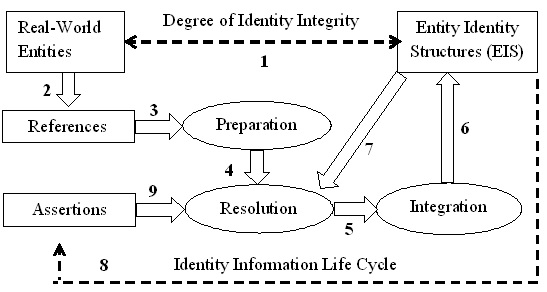
\includegraphics[width=14cm,height=7cm]{Figures/OriginalEIIM.jpg}
%\end{figure} 
%
%In this section we explain the current EIIM process that lays the foundation and acts as a background of the presented research.
%The idea of Entity Identity Information Management (EIIM) as defined by [15] is the collection and management of identity information of real-world entities with the goal of sustaining entity identity integrity. Their model of EIIM was motivated by the problem of entity resolution in information systems, particularly in the domain of MDM (Master Data Management). They define entity resolution as the process of determining whether two references to real-world objects in an information system are referring to the same object, or to different object [16]. The EIIM life cycle as proposed by them is an iterative process that combines entity resolution and data structures representing entity identity into specific operational configurations (EIIM configurations, as shown in Figure 3), that when executed in concert, work to maintain the entity identity integrity of master data over time. The EIIM framework is implemented by developing open source software known as OYSTER .

